\section{Machine Learning}

\subsection{Introduction}

\againframe<4-5>{overview}
%TODO: more machine learning examples (decision tree, ....)
%TODO: neuronal nets erklären

%TODO: RNN new graphic

\begin{frame}{Introduction}{Supervised and Unsupervised learning}
    \begin{table}
        \def\arraystretch{1.5}
        \scriptsize
        \begin{tabular}{r | p{.3\textwidth} | p{.3\textwidth}}
            & Supervised & Unsupervised \\
            \hline
            Learning Data & \tabitem input X &  \tabitem input X\\
            & \tabitem target values Y & \\
            What is learned & mapping function $Y \approx f(X)$ & model of data structure\\
            Examples & \tabitem classification & \tabitem clustering \\
            & \tabitem regression & \tabitem association \\
        \end{tabular}
    \end{table}

    \notes{
        \item warum machine learning (und nicht vorgegebene gesten erkennen)
        \item supervised unsupervised
        \item vorteile/ nachteile
        \item warum supervised
    }
\end{frame}

\subsection{Neural Networks}
\begin{frame}{Neural Networks}{Strengths and Weaknesses \cite{tu-advantages-disadvantages-neural-networks}}
    \begin{columns}
        \begin{column}{0.5\textwidth}
            \textbf{Pros}
            \begin{itemize}
                \item general-purpose
                \item many variations
                \item fast to apply once learned
                \item able to detect complex relationships
            \end{itemize}
        \end{column}
        \begin{column}{0.5\textwidth}
            \textbf{Cons}
            \begin{itemize}
                \item requires large dataset
                \item blackbox\footnotemark[1], difficult to ``understand''
                \item slow to learn
                \item can overfit
            \end{itemize}
        \end{column}
    \end{columns}

    \footnotetext[1]{there are some rule-extraction algorithms \cite{web:misconceptions-neural-network}}


    \notes{
        \item \textbf{ARE }general-purpose
        \item easiliy generate data
        \item not important how (we dont know movement of fingers)
        \item tradeoff: complex calculation <-> data needed to learn
        \item bridge: NN we were interested in
    }
\end{frame}

\subsection{Recurrent Neural Networks}
\begin{frame}{Recurrent Neural Networks}
    \centering
    \vfill
    \begin{figure}
        \begin{tikzpicture}[
    ->,
    >=stealth',
    shorten >=1pt,
    auto,
    node distance=2.2cm,
    semithick,
    layer/.style={
        draw,
        minimum width=0.9cm,
        minimum height=6cm,
    },
    bend angle=15,
    every state/.style={
        very thick,
        fill=white,
        distance=1.2,
        minimum size=0.5cm,
    },
]
    \node[state]         (D)  {};
    \node[state]         (A) [above left=1cm and 2.2cm of D] {};
    \node[state]         (B) [below left=1cm and  2.2cm of D] {};

    \node[state]         (C) [above of=D] {};

    \node[state]         (E) [below of=D] {};
    \node[state]         (F) [right =2.2cm of D] {};

    \path   (A) edge              node {} (C)
                edge              node {} (D)
                edge              node {} (E)

              (B) edge              node {} (C)
                edge              node {} (D)
                edge              node {} (E)

            (C) edge [loop above,gray] node {} (C)
                edge              node {} (F)
                edge [bend left,gray]  node {} (D)
                edge [bend left,gray]  node {} (E)

            (D) edge [loop above,gray] node {} (D)
                edge              node {} (F)
                edge [bend left,gray]  node {} (C)
                edge [bend left,gray]  node {} (E)

            (E) edge [loop above,gray] node {} (E)
                edge [bend left,gray]  node {} (C)
                edge [bend left,gray]  node {} (D)
                edge              node {} (F);


    \node[layer,label=below:{\small\textbf{input}}] at ($(A) !.5! (B)$) {};
    \node[layer,label=below:{\small\textbf{hidden}}] at (D) {};
    \node[layer,label=below:{\small\textbf{output}}] at (F) {};
    % \draw ($(E.south west) - (0.2, 0.2)$) rectangle ($(C.north east) + (0.2, 0.2)$);
    % \draw ($(F.south west) - (0.2, 0.2)$) rectangle ($(F.north east) + (0.2, 0.2)$);

\end{tikzpicture}

        \caption{Simplified Recurrent Network}
        \label{fig:recurrent-network}
    \end{figure}
    \notes{
        \item sequences of data, not necessarily same length
        \item dependencies between data
        \item ie handwriting, language recognition, driverless cars, accident prediction
        \item forecast
        \item Aufbau
        \item Vanishing Gradient Problem
    }
\end{frame}
\subsection{Problems}
\begin{frame}{Problems}{Vanishing Gradient Problem (\citet{hochreiter-vanishing-gradient})}
    \vfill\null
    \begin{block}{Problem}
        Deep networks require a lot of training
        \uncover<2->{
            \begin{itemize}
                \item during backpropagation, error is lost with each layer
                \item first layers receive slowest updates
                \item unrolled RNNs are very deep
            \end{itemize}
        }
    \end{block}
    \vfill\null
\end{frame}
% \begin{frame}{Evaluating Predictions}{Imbalanced Data}
%     \begin{itemize}
%         \item 2\% keystrokes $\rightarrow$ positive class
%         \pause
%         \item one class predictions
%         \pause
%         \item cost function needs to counteract
%     \end{itemize}
% \end{frame}
\begin{frame}{Problems}{Imbalanced Data}
    \vfill\null
    \begin{block}{Problem}
        Only 2\% of our samples are keystrokes (positive class)
    \end{block}
    \pause
    \vfill\null
    \begin{block}{Possible solutions \citep{web:combat-imbalanced-dataset}}
        \begin{itemize}
            \item gather lots of data and train a lot
            \item resampling
            \item penalize
            \item generate synthetic data
        \end{itemize}
    \end{block}
    \vfill\null

    \notes{
        \item fast!
        \item Problems with RNN!
        % \item 8 ways to...
        \item oversampling, undersampling
        \item penalize choosing neg class wrongly
        \item for theoratical math problems
        \item SOLUTION: not RNN
        \item \textbf{Look at actual data}
    }
\end{frame}

\begin{frame}{Preprocessing and Sampling}
    \begin{columns}[T]
        \begin{column}{0.3\textwidth}
            \begin{figure}
                \begin{tikzpicture}[
    node distance=5mm,
    node/.style={
        flowchart node,
        minimum width=2cm,
        text width=2cm,
    },
    highlight/.style={
        draw=primary,
        color=primary,
        fill=primary!10!white,
    },
]
    \node[node,onslide={<2-3> highlight}]  (quat) at (0, 0) {Quaternions};
    \node[node,onslide={<2-3> highlight}, below=of quat] (rel) {Relative to base};
    \node[node,onslide={<4> highlight}, below=of rel] (int) {Timesteps/\\Interpolate};
    \node[node,onslide={<5> highlight}, below=of int] (samples) {Pick samples at key strokes};
    \node[node,onslide={<5> highlight}, below=of samples,dashed] (angles) {Extract angles for visualization};

    \draw[flowchart arrow] (quat) -- (rel);
    \draw[flowchart arrow] (rel) -- (int);
    \draw[flowchart arrow] (int) -- (samples);
    \draw[flowchart arrow,dashed] (samples) -- (angles);
\end{tikzpicture}

            \end{figure}
        \end{column}
        \begin{column}{0.7\textwidth}
            \only<2>{
                \begin{figure}
                    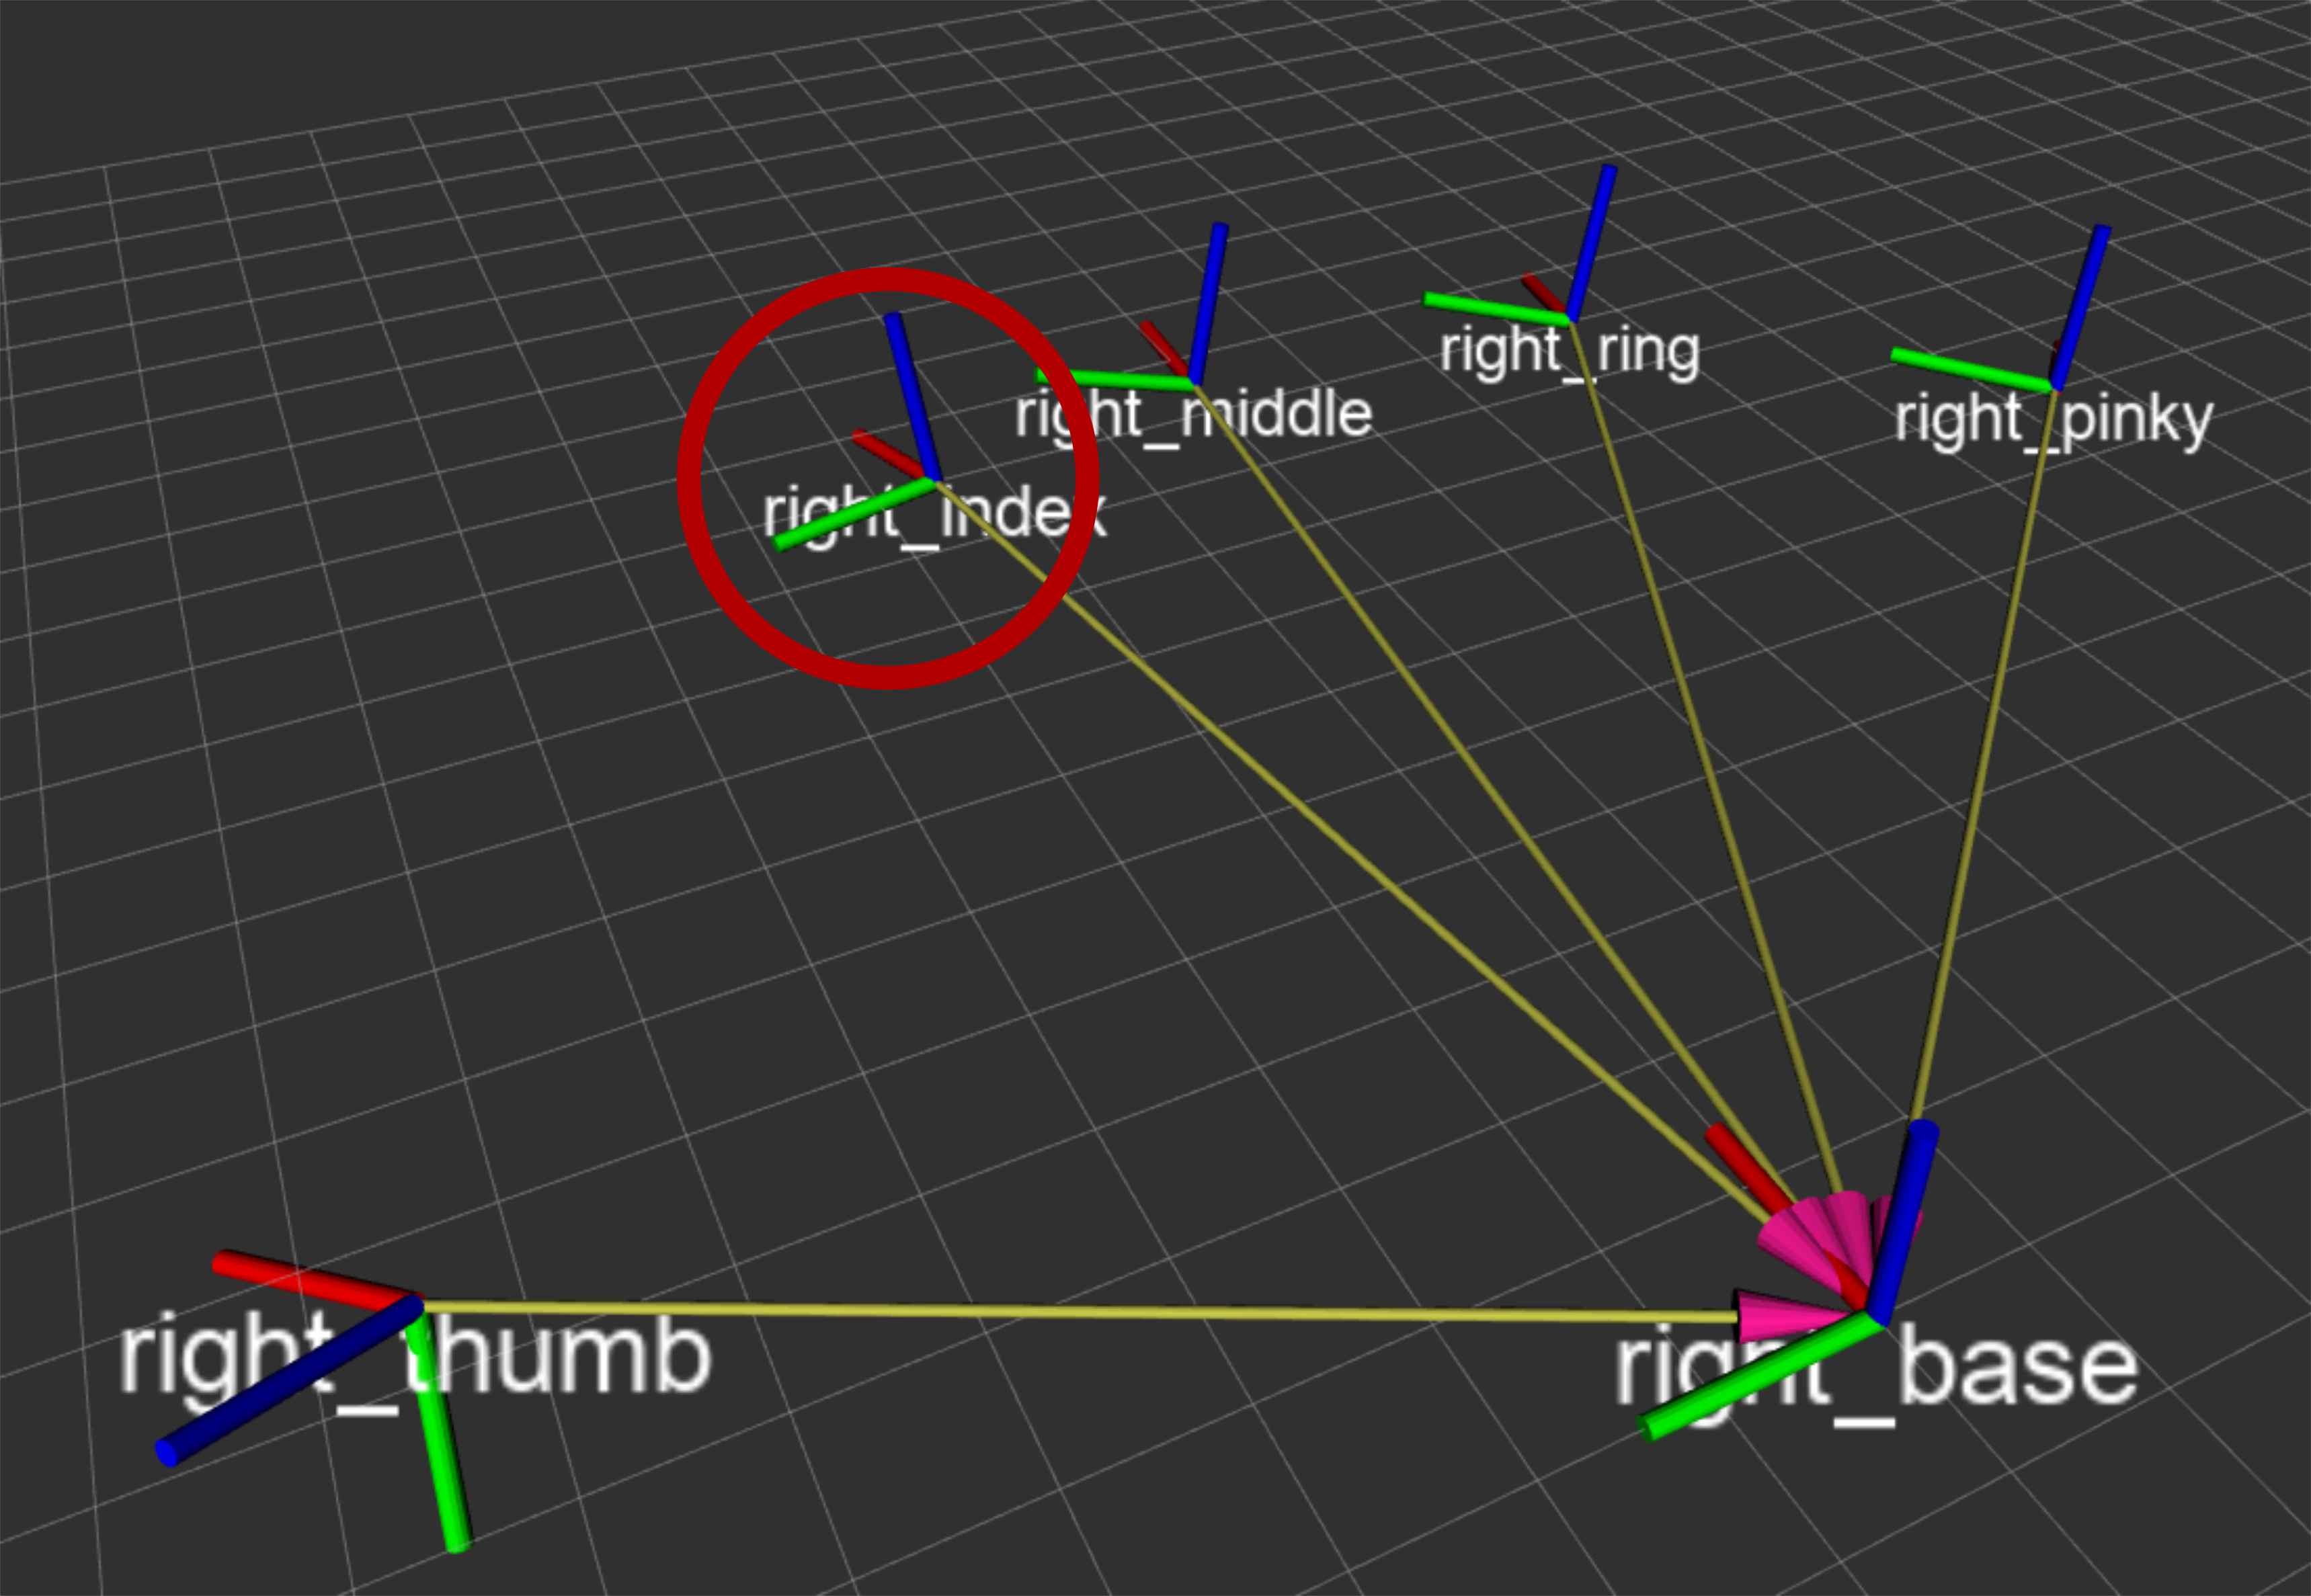
\includegraphics[width=\textwidth]{../common/images/rviz-idle-pose}
                    \caption{Visualization of relative quaternion rotations, idle pose}
                \end{figure}
            }
            \addtocounter{figure}{1}
            \only<3>{
                \begin{figure}
                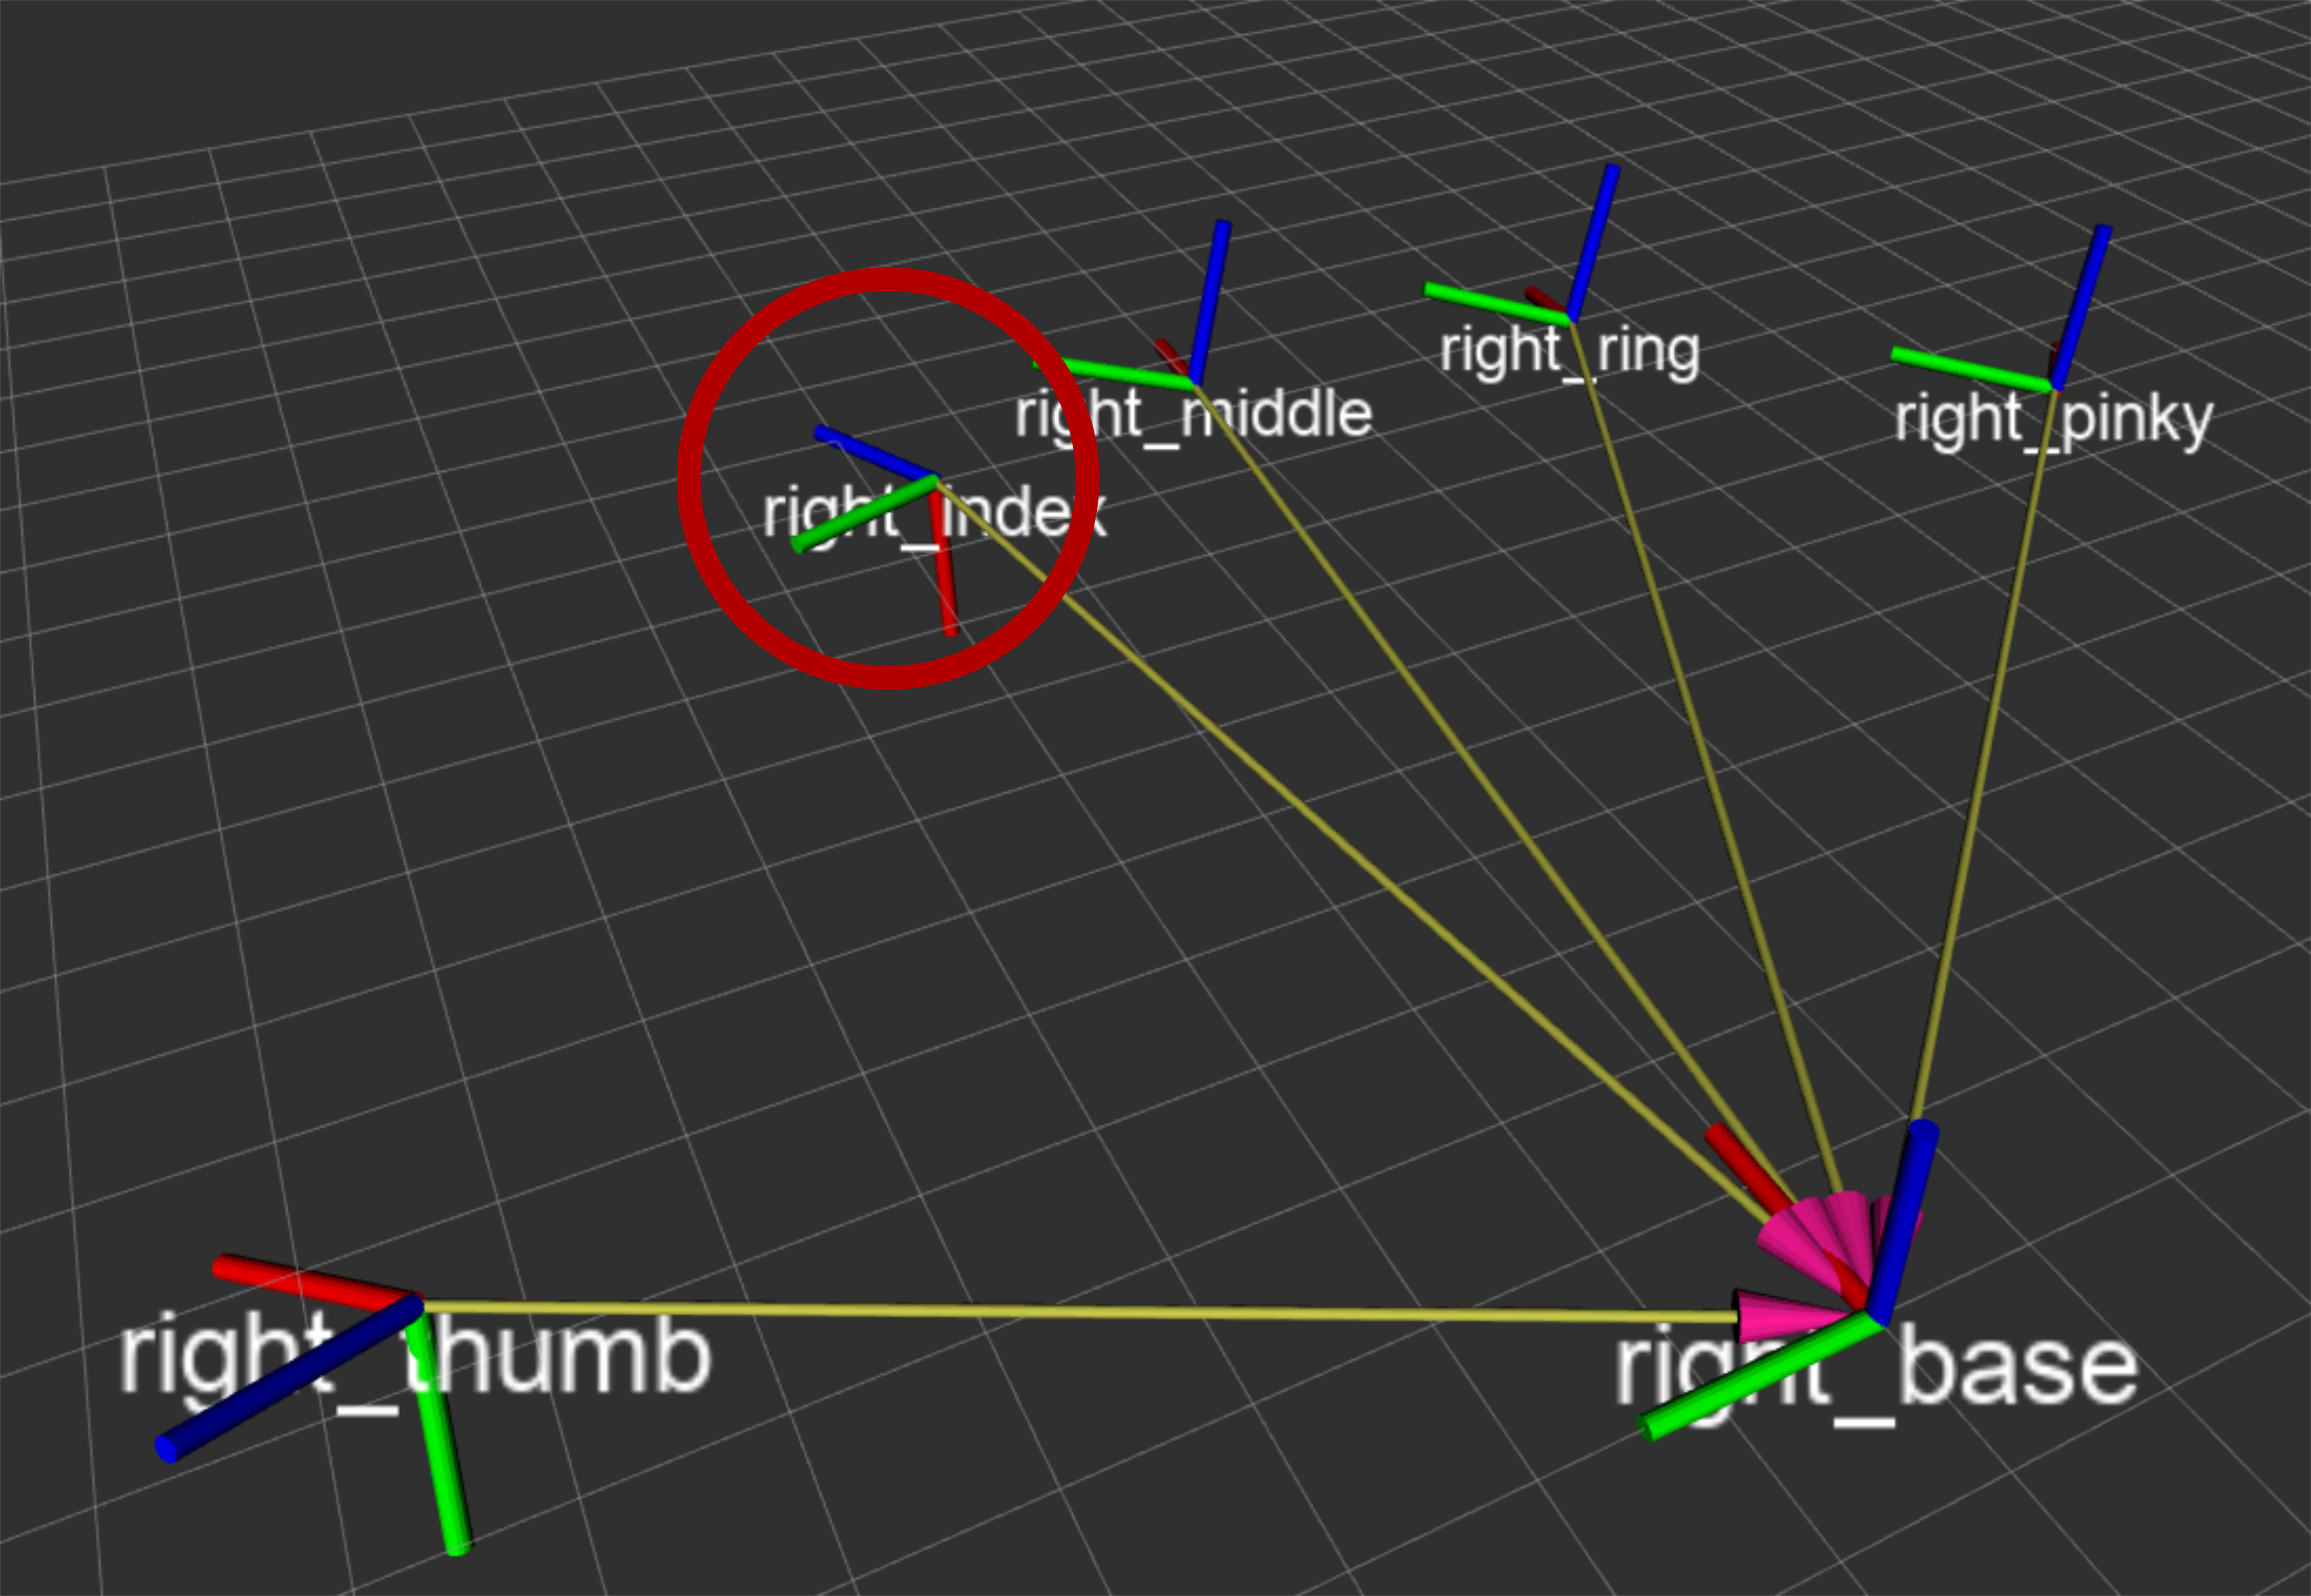
\includegraphics[width=\textwidth]{../common/images/rviz-index-finger-bent}
                    \caption{Visualization of relative quaternion rotations, index finger bent}
                \end{figure}
            }
            \addtocounter{figure}{1}

            \only<4> {
                \begin{figure}
                    \begin{tikzpicture}[
    curve/.style={
        mark=x,
        mark options={thick},
        mark size=3pt,
        thick,
    },
    dot/.style={
        minimum width=4pt,
        minimum height=4pt,
        inner sep=0pt,
        circle,
        draw=secondary,
        thick,
    },
]
    \begin{axis}[
        width=12cm,
        height=6cm,
        axis x line=center,
        axis y line=center,
        xmin=2, xmax=7,
        ymin=2, ymax=5,
        xlabel=Zeit, xtick style={draw=none}, xtick=\empty,
        ylabel=Wert, ytick style={draw=none}, ytick=\empty,
        xlabel near ticks,
        ylabel near ticks,
        legend columns=-1,
        legend style={
            at={(0.5,1.1)},
            anchor=south,
            draw=none,
            font=\scriptsize\bfseries,
            text width=3em,
            text height=1.5ex,
            text depth=.5ex,
        },
    ]
        \addplot[curve,name path=imu-1,color=plot0] plot coordinates {
(-1.90, 1.78) (-1.40, 2.09) (-0.90, 2.32) (-0.40, 2.45) (0.10, 2.58) (0.60, 2.87) (1.10, 3.01) (1.60, 3.01) (2.10, 2.89) (2.60, 2.96) (3.10, 3.05) (3.60, 2.97) (4.10, 2.81) (4.60, 2.77) (5.10, 2.72) (5.60, 2.64) (6.10, 2.49) (6.60, 2.48) (7.10, 2.67) (7.60, 2.81) (8.10, 3.10) (8.60, 3.31) (9.10, 3.48) (9.60, 3.70) (10.10, 3.88) (10.60, 4.05) (11.10, 4.35) (11.60, 4.50)
        };
        \addlegendentry{IMU~1}

        \addplot[curve,name path=imu-2,primary,color=plot1] plot coordinates {
(-1.68, 4.84) (-1.18, 4.89) (-0.68, 4.82) (-0.18, 4.62) (0.32, 4.46) (0.82, 4.13) (1.32, 3.88) (1.82, 3.81) (2.32, 3.71) (2.82, 3.49) (3.32, 3.45) (3.82, 3.24) (4.32, 3.19) (4.82, 3.20) (5.32, 3.24) (5.82, 3.09) (6.32, 2.77) (6.82, 2.62) (7.32, 2.39) (7.82, 2.26) (8.32, 2.32) (8.82, 2.32) (9.32, 2.47) (9.82, 2.55) (10.32, 2.47) (10.82, 2.23) (11.32, 1.92) (11.82, 1.46)
        };
        \addlegendentry{IMU~2}


        \foreach \x/\s [count=\i] in {3.5/2-, 1.5/3-, 5.5/3-, 7.5/3-} {
            \addplot [secondary, name path=line-\i] coordinates{(\x, -0.5) (\x, 5)};

            \path[name intersections={of=imu-1 and line-\i,by=I-\i}];
            \node[dot] at (I-\i) {};

            \path[name intersections={of=imu-2 and line-\i,by=J-\i}];
            \node[dot] at (J-\i) {};
        }

        \draw[secondary,thick,<->]
            (axis cs:3.5,4.6)
                -- node[above] {\tiny{}fester Zeitschritt}
                node[below] {\tiny{}($25$ Hz)}
                (axis cs:5.5,4.6);
    \end{axis}
\end{tikzpicture}

                    \label{fig:interpolation}
                    \caption{Interpolation of the IMU data (simplified)}
                \end{figure}
            }
            \addtocounter{figure}{1}

            \only<5>{
                \vfill\null
                \begin{figure}
                    \centering
                    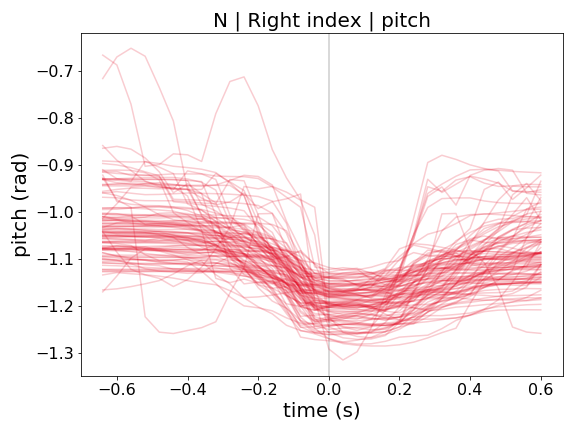
\includegraphics[width=0.8\textwidth]{../common/images/plot-samples-1x1}
                    \caption{Multiple repetitions of the N key stroke, overlayed at the moment of pressing the key (center line); value plotted
                    is extracted relative pitch angle of right index finger.}
                \end{figure}
                \vfill\null
            }
            \addtocounter{figure}{1}

            % Sampling
            % \begin{itemize}
            %     \item 25 Hz timesteps
            %     \item 16 timesteps per sample
            %     \item key stroke in center
            %     \item 100 samples per epoch
            % \end{itemize}
        \end{column}
    \end{columns}

    \note{
        \begin{enumerate}
            \item Quat:
            \begin{itemize}
                \item absolute orientation (heading north)
                \item goal: independent of direction
                \item solution: use relative quaternions (handbase)
                \item hand relative to moving average
                \item $$q_{rel} = q_{abs} \cdot inv(q_{abs,parent})$$
            \end{itemize}
            \item interpolate
            \begin{itemize}
                \item fixed timesteps
                \item need all imu data
            \end{itemize}
            \item sampling
            \begin{itemize}
                \item time 0 : keystroke
                \item 8 timesteps before + after
                \item visualization: many keystrokes, angles \textbf{yaw, pitch}
            \item acceleration (linear acceleration)
            \item gyroscope (angular velocity (rotate speed))
            \item (spherical) linear interpolation $\rightarrow$ see next slide
            \end{itemize}
        \end{enumerate}
    }
\end{frame}

\begin{frame}{Preprocessing and Sampling}{Real Preprocessed Data}
    \phasekeyboard{1}
    \vspace{-1em}
    \begin{figure}
        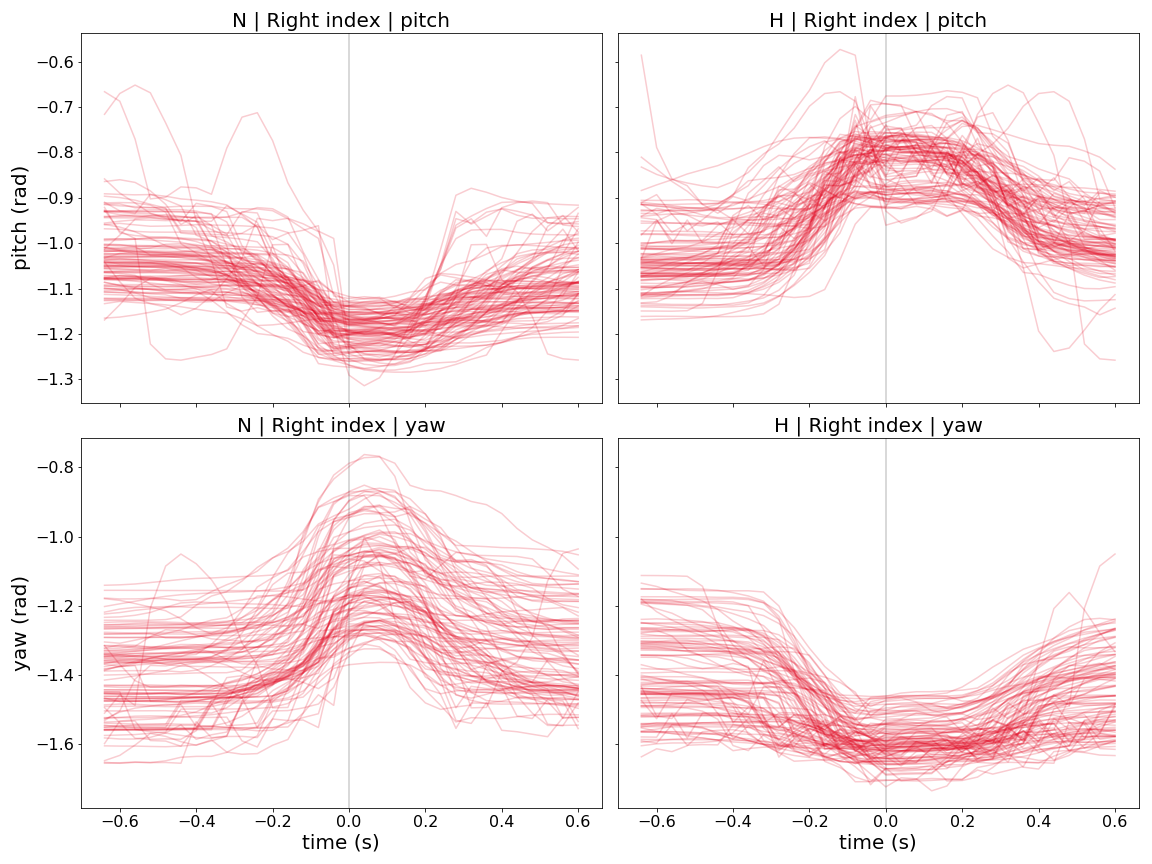
\includegraphics[width=0.65\textwidth]{../common/images/plot-samples-2x2}
        \label{fig:our_data}
        \caption{Multiple repetitions of N (\emph{left}) and H (\emph{right})
        key strokes, overlayed at the moment of pressing the key (center line);
        value plotted is extracted relative pitch (\emph{top})/yaw
        (\emph{bottom}) angles of right index finger.}
    \end{figure}

    \notes{
        \item we tried to visualize what we got
        \item 1 finger, left: N, right: H
        \item Quaternion: yaw, pitch
        \begin{itemize}
            \item quat is enough, acc and gyro data can be used additionally $\rightarrow$ requires more training
            \item finger cant roll relative to hand $\rightarrow$ no roll necessary (only hand)
        \end{itemize}
        \item actual moment of keystroke!
        \item hill, valley!
        \item visibly different --> detectible!!
    }
\end{frame}

\subsection{Convolutional Neural Networks}
\begin{frame}[fragile]{Convolutional Neural Networks}{Convolution and Pooling}
    \begin{figure}
        \begin{tikzpicture}
    \matrix(start)[
        matrix of nodes,
        inner sep=0pt,
        draw,
        nodes={
            inner sep=0pt,
            text width=.5cm,
            align=center,
            minimum height=.5cm,
            draw,
        }
    ]{
       5  & 2 & 3 & 8 \\    0 & |[fill=primary!25]|{1} & 2 & 6 \\    4 & 8 & 5 & 4 \\    1 & 7 & 1 & 7\\};

    \matrix(filter0)[
        inner sep=0pt,
        draw,
        label=above:{\tiny{}Filter 0},
        opacity=0.5,
        above right=-0.2cm and 0.8cm of start,
        matrix of nodes,
        nodes={
            inner sep=0pt,
            text width=.5cm,
            align=center,
            minimum height=.5cm,
            draw,
        },
    ]{
        0 & 1 & 0 \\    0 & 1 & 0 \\    0 & 1 & 0 \\};
    \matrix(filterN)[
        inner sep=0pt,
        draw,
        label=above:{\tiny{}Filter N},
        opacity=0.5,
        below right=-0.2cm and 0.8cm of start,
        matrix of nodes,
        nodes={
            inner sep=0pt,
            text width=.5cm,
            align=center,
            minimum height=.5cm,
            draw,
        },
    ]{
        0 & 0 & 1 \\    0 & 1 & 0 \\    1 & 0 & 0 \\};

    \node (rect) at (-0.25, 0.25) [draw=primary,line width=0.6mm,minimum width=1.5cm,minimum height=1.5cm] {};
    \draw[->, thick, primary] (rect) -- (filter0);
    \draw[->, thick, primary] (rect) -- (filterN);

    \matrix(conv0)[
        matrix of nodes,
        inner sep=0pt,
        draw,
        right=of filter0,
        label=above:{\tiny{Feature Map 0}},
        nodes={
            inner sep=0pt,
            text width=.5cm,
            align=center,
            minimum height=.5cm,
            draw,
        }
    ]{
        5 & 3 & 5 & 14 \\    9 & |[fill=primary!25]|{11} & 10 & 18 \\    5 & 16 & 8 & 17 \\    5 & 15 & 6 & 11\\};

    \matrix(convN)[
        matrix of nodes,
        inner sep=0pt,
        draw,
        right=of filterN,
        label=above:{\tiny{}Feature Map N},
        nodes={
            inner sep=0pt,
            text width=.5cm,
            align=center,
            minimum height=.5cm,
            draw,
        }
    ]{
        5 & 2 & 4 & 10 \\    2 & |[fill=primary!25]|{8} & 18 & 11 \\    5 & 11 & 18 & 5 \\    9 & 12 & 5 & 7\\};

    \node (rect2) at ($(conv0) + (-0.5, 0.5)$) [draw=orange,line width=0.6mm,minimum width=1cm,minimum height=1cm] {};
    \node (rect2) at ($(convN) + (-0.5, 0.5)$) [draw=orange,line width=0.6mm,minimum width=1cm,minimum height=1cm] {};
    \matrix(pool0)[
        inner sep=0pt,
        draw,
        label=above:{\tiny{}Pool 0},
        right=of conv0,
        matrix of nodes,
        nodes={
            inner sep=0pt,
            text width=.5cm,
            align=center,
            minimum height=.5cm,
            draw,
        },
    ]{
        |[fill=orange!25]|{11} & 18 \\    16 & 17 \\};
    \matrix(poolN)[
        inner sep=0pt,
        draw,
        label=above:{\tiny{}Pool N},
        right=of convN,
        matrix of nodes,
        nodes={
            inner sep=0pt,
            text width=.5cm,
            align=center,
            minimum height=.5cm,
            draw,
        },
    ]{
        |[fill=orange!25]|{8} &  18\\    12 & 18 \\};
    % \draw(rect)[primary, line width=0.65mm] (-1,-0.5) rectangle (0.5,1);
    \draw[->, line width=1pt, primary,bend angle=20] (filter0.east |- conv0-2-2.north west) to[bend left] (conv0-2-2.north west);
    \draw[->, line width=1pt, primary,bend angle=20] (filterN.east |- convN-2-2.north west) to[bend left] (convN-2-2.north west);
    \draw[->, line width=1pt, orange,bend angle=20] (conv0-2-2.east |- pool0-1-2.north west) to[bend left] (pool0-1-1.north west);
    \draw[->, line width=1pt, orange,bend angle=20] (convN-2-2.east |- poolN-1-2.north west) to[bend left] (poolN-1-1.north west);
    \node[font=\Large] at ($(filter0)!0.45!(filterN)$) {$\vdots$};
    % \path   (rect) edge              node {} (filter0)
            % (rect) edge              node {} (filterN);

    \node[font=\Large] at ($(conv0)!0.45!(convN)$) {$\vdots$};
\end{tikzpicture}

        \label{fig:cnn}
        \caption{Feature Extraction with CNN}
    \end{figure}

    \notes{
        \item convolute (element wise multiplication)
        \item pool (max)
        \item filters (50)
        \item 3 x 3 x 50
        \item convolute, pool..
        \item fully connected layer as classifier
    }
\end{frame}

\begin{frame}[fragile]{Convolutional Neural Networks}{Our Implementation}
    \vspace{-1em}
    \begin{tikzpicture}[
    node distance=5mm,
    io/.style={
        flowchart node,
        minimum height=0.5cm,
        text width=1cm,
        minimum width=0cm,
    },
    arrow/.style={
        flowchart arrow,
    },
    arrow/.style={
        ->,
        >=stealth',
        shorten >=1pt,
        auto,
        semithick,
    },
    layer/.style={
        draw,
        minimum width=0.9cm,
        minimum height=6cm,
    },
    bend angle=15,
    every state/.style={
        fill=white,
        minimum size=3mm,
        inner sep=0pt,
        node distance=7mm,
    },
    steplabel/.style={
        font=\scriptsize,
        above,
        rotate=90,
        anchor=west,
    },
]
    \node[io] (data) {1 @\\16 x 24};
    \node[io, right=of data] (conv1)  {50  @\\$16 \times 24$};
    \node[io, right=of conv1] (pool1) {50   @\\$8 \times 12$};
    \node[io, right=of pool1] (conv2) {50 @\\$8 \times 12$};
    \node[io, right=of conv2] (pool2) {50 @\\$4 \times 6$};
    \node[io, right=of pool2] (hidden) {Hidden\\Layer};
    \node[io, right=of hidden] (out) {Output\\Layer};

    \draw [arrow] (data)   -- node[steplabel] {conv 1} (conv1);
    \draw [arrow] (conv1)  -- node[steplabel] {pool 1} (pool1);
    \draw [arrow] (pool1)  -- node[steplabel] {conv 2} (conv2);
    \draw [arrow] (conv2)  -- node[steplabel] {pool 2} (pool2);
    \draw [arrow] (pool2)  -- node[steplabel] {dense} (hidden);
    \draw [arrow] (hidden) -- node[steplabel] {dense} (out);
\end{tikzpicture}

    \notes{
        \item each key has same amount of samples
        \item one sample = one keystroke
        \item filter randomly initialized
        \item filter are learned!
        \item matrix with numbers instead of color scheme
        \item 2 x convolute and pooling
        \item MSE: $(1/n)*\sum_{n=0}^{N} (pred - act)^2$
            % \begin{itemize}
            %     \item Input: relative angles of quaternions
            %      \item Hand Imu: relative to last position
            %     \item 50 3x3 Filter
            %     \item 2 Iterations
            %     \item fully connected layer
            %     \item N units in output layer ($N=count of keys$)
            %     \item costfunction: Mean Squared Error
            % \end{itemize}
    }
\end{frame}
\subsection{Evaluating Predictions}


\addtocontents{toc}{\newpage}

